\chapter{Special topics}\label{chMarkov}
In this chapter we delve into some fun, modern, and more advanced topics in statistics: algebraic statistics, entropy, likelihood, Markov chains, and information criteria.
\label{hmc}

\section{Algebraic statistics}\label{sec:algebraic}

Consider two Bernoulli random variables $X$ and $Y$, both with parameter $p$.
We can define four numbers $p_{00}, p_{01}, p_{10}, p_{11}$ by
\[
	p_{ij}=\P(X=i\text{ and }Y=j).
\]
Let us write $q=p_{1,1}$. It might be that $\P(X=Y)=1$, in which case $q=p$.
It might also be that $\P(X=1-Y)=1$, in which case $q=0$. So it seems that $q$ can vary, with $0\le q\le p$.
On the other hand, $q$ determines the other parameters $p_{00}, p_{01}, p_{10}$, as can be seen from the following table:
\[
\begin{tabular}{c|c|c|c}
		& $X=0$		& $X=1$		& $X\in\{0,1\}$\\
\hline
$Y=0$	& $p_{00}$	& $p_{10}$	& $p_{+0}=1-p$	\\
$Y=1$	& $p_{01}$	& $p_{11}$	& $p_{+1}=p$	\\
\hline
$Y\in\{0,1\}$	& $p_{0+}=1-p$	& $p_{1+}=p$	& $p_{++}=1$
\end{tabular}
\]
Indeed, the only solution is
\[
\begin{tabular}{c|c|c|c}
		& $X=0$		& $X=1$		& $X\in\{0,1\}$\\
\hline
$Y=0$	& $p_{00}=1-p-(p-q)$	& $p_{10}=p-q$	& $p_{+0}=1-p$	\\
$Y=1$	& $p_{01}=p-q$	& $p_{11}=q$	& $p_{+1}=p$	\\
\hline
$Y\in\{0,1\}$	& $p_{0+}=1-p$	& $p_{1+}=p$	& $p_{++}=1$
\end{tabular}
\]
The value for $p_{00}$ implies another constraint on $q$:
\[
	2p-1\le q.
\]
Indeed, these numbers then must satisfy some equations: they must be nonnegative, and:
\[
	p_{00}+p_{01}=1-p\quad\text{since $\P(X=0)=1-p$}
\]
\[
	p_{10}+p_{11}=p\quad\text{since $\P(X=1)=p$}
\]
\[
	p_{00}+p_{10}=1-p\quad\text{since $\P(Y=0)=1-p$}
\]
\[
	p_{01}+p_{11}=p\quad\text{since $\P(Y=1)=p$}
\]
The fact that all the $p_{ij}$ add up to 1 follows.
How much variability remains? What are all the joint distributions $X$ and $Y$ can have?
Well, let
\[
	q=\P(X=1\text{ and }Y=1).
\]
Then $\P(X=1\text{ and }Y=0)=p-q=\P(X=0\text{ and }Y=1)$, and $\P(X=0\text{ and }Y=0)=1-p-(p-q)$.
So we have a 1-dimensional family of joint distributions.
When $q=0$, we have $\P(X=1-Y)=1$. When $q=p$, we have $\P(X=Y)=1$.
Moreover, the constraint on $q$ is that $0\le q\le p$ and $p-q\le 1-p$, i.e., $q\ge 2p-1$.
In a sense, the joint distributions for fixed $p$ form a parametrized curve in $\mathbb R^4$.\footnote{For much more on algebraic statistics, see Seth Sullivant, Algebraic Statistics, \emph{Graduate Studies in Mathematics} \textbf{194}, 2018.}


As another example, we consider phylogenetic trees.
The spike protein of a SARS-CoV-2 virus contains $n=1273$ amino acids.
The famous D614G mutation involved a change in position 614.
Assume the positions are independent random variables that change value with time.
Which value of $p$ will maximize the probability of exactly $k=1$ changes occurring? That is,
\[
	L(p) = \binom{n}{k} (1-p)^{n-k}p^k
\]
We take the derivative with respect to $p$, after first taking the logarithm:
\[
	\ln L(p) = \ln \binom{n}{k} + (n-k)\ln(1-p) + k\ln p
\]
\[
	0 =^! \frac{d}{dp}\ln L(p) = \frac{k}p - \frac{n-k}{1-p}
\]
\[
	\frac{k}p = \frac{n-k}{1-p}
\]
\[
	k(1-p)=(n-k)p
\]
\[
	np = k 
\]
\[
	p = k/n = 1/1273
\]
Then $L(p)=1273 (1272/1273)^{1272}/1273 = (1-1/1273)^{1272}\approx 1/e\cdot (1-1/1273)\approx 1/e$.
Then the probability of just the D614G change (amino acid D changes into amino acid G in position 614) is approximately $\epsilon := 1/(1273\cdot 20\cdot e)$ where $20$ is the number of possible choices for an amino acid.

Now consider the following mutations.
\begin{verbatim}
   Position                     5    74   88   439  520  614  797  1176 1263
 1 YP_009724390 Wuhan RefSeq    L    N    D    N    A    D    F    V    P
 2 QIC53204 Sweden February 7   L    N    D    N    A    D    C    V    P
 3 QKT21230 Hawaii March 12     L    N    D    N    A    G    F    V    P
 4 QJU70329 Alaska March 24     L    N    A    N    A    G    F    V    P
 5 QJU70425 Alaska March 25     L    N    D    N    A    G    F    V    L
 6 QJU70545 Alaska April 26     L    N    D    N    S    G    F    V    P
 7 QIZ15981 Nevada March 9      F    N    D    N    A    D    F    V    P
 8 QLM06051 Illinois July 7     L    N    D    K    A    G    F    V    P
 9 QLF80256 Brazil March 20     L    N    D    N    A    G    F    F    P
10 QJA41641 Brazil March 18     L    K    D    N    A    D    F    V    P
\end{verbatim}
It is given that the Wuhan Reference Sequence is the root of our phylogenetic (inheritance) tree.
Moreover, the Hawaii sequence has the D614G mutation.
Sequences that differ from Wuhan RefSeq by one mutation, but not in position 614, are:
Sweden, Nevada, BrazilMarch18.
Sequences that differ from the Hawaii sequence in one position, but not in position 614, are:
AlaskaMarch24, AlaskaMarch25, AlaskaApril26, Illinois, BrazilMarch20.
It is ``obvious'' that the tree should now be:
\begin{verbatim}
Wuhan RefSeq: root
Hawaii, Sweden, Nevada, BrazilMarch18: children of the root
AlaskaMarch24, AlaskaMarch25, AlaskaApril26, Illinois, BrazilMarch20: children of Hawaii
\end{verbatim}
This could be made precise by asking: which tree structure maximizes the relevant probability?
For our ``obvious'' tree the probability is $\epsilon^9$ as each node differs in only one position from its parent.
On the other hand, if we made a linear tree with Wuhan at the root and BrazilMarch18 at the leaf, we would need
$\epsilon^{1+2+1+2+2+3+3+2+3}=\epsilon^{19}$ since Sweden differs from Wuhan in 1 position, then Hawaii from Sweden in 2 positions, and so on.

In general, the probability associated with a tree is the product of probabilities along its edges.


In this virus example, it is plausible, or even convincing, that the ancestors of viruses in the data set are all also in the data set (except for the ancestors of the Wuhan virus).
In other examples this is not so.
Consider the following example from Sullivant.
\begin{verbatim}
Chimp    ACCTTGGAAGGTAAACGA
Human    ACCGTGCAACGTGAACGA
Gorilla  ACCGTGCAACGTAAACTA
\end{verbatim}
The fewest differences are 2 between Human and Gorilla.
In both cases, where Human and Gorilla differ, one of them agrees with Chimp.
This suggests a hypothetical common ancestor of Human and Gorilla given by
\begin{verbatim}
Ancestor ACCGTGCAACGTAAACGA
\end{verbatim}
This makes the distance Ancestor to Human 1, and Ancestor to Gorilla 1.
The distance from Ancestor to Chimp is 3.
Now we may wonder if there is one common ancestor
\begin{verbatim}
Common ACC?TG?AA?GTAAACGA
\end{verbatim}

to Ancestor and Chimp, or whether Chimp evolved from Ancestor as well.
Let us consider these two models.
With the common ancestor, the probability is a sum over all possible values for the three question marks ???:
\begin{verbatim}
??? Probability
AAA epsilon^6
AAC epsilon^5
AAG epsilon^5
AAT epsilon^6
...
\end{verbatim}
Notice that Chimp has ???=TGG and Ancestor has ???=GCC.

For instance, if the common ancestor has ???=AAA then to evolve into Chimp and Ancestor gives a factor of $\epsilon^{3+3}$.
There will be $2^3$ choices with $\epsilon^6$ (nothing in common with TGG nor GCC).
Let us use 0 for a symbol not in common with either and 1 for a symbol in common with one of them. Then the possibilities are
000 for a probability $8\cdot \epsilon^6$;
001,010,100 for a total probability $3\cdot 8\cdot \epsilon^5$;
011, 101, 110 for a total probability $3\cdot 8\cdot \epsilon^4$;
111 for a probability $8\cdot \epsilon^3$;
for a total of
\[
	8 \epsilon^6 + 24 \epsilon^5 + 24 \epsilon^4 + 8\epsilon^3 = 8\epsilon^3(\epsilon^3+3\epsilon^2+3\epsilon+1)=8\epsilon^3(\epsilon+1)^3
\]


Without the common ancestor, there is no such sum and the probability is just $\epsilon^{3}$.

So we see that the 5-species tree gives a higher probability than the 4-species tree.

This is not quite right, however, since $\epsilon$ was the probability of exactly one change.
%\includegraphics{ch_markov/figures/wolfram-s4cs.png}
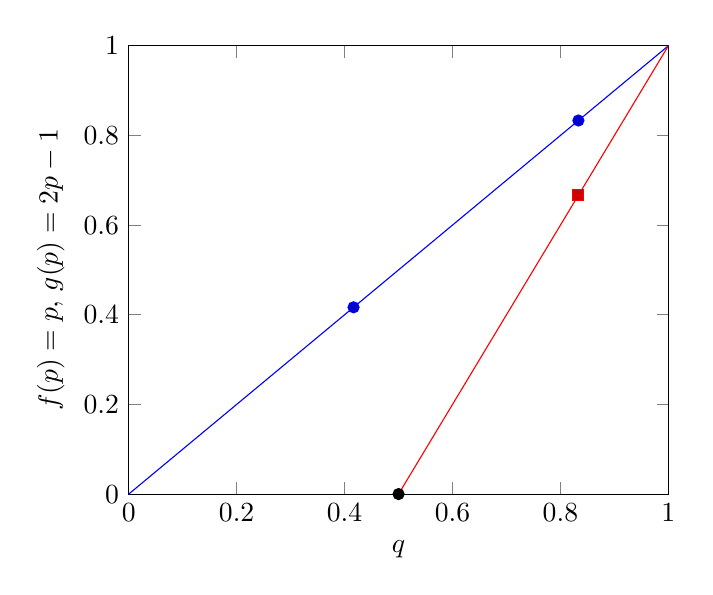
\begin{tikzpicture}
  \begin{axis}[ 
	xmin=0,   xmax=1,
	ymin=0,   ymax=1,
    xlabel=$q$,
    ylabel={$f(p) =p$, $g(p)=2p-1$}
  ] 
    \addplot {x}; 
    \addplot{2*x-1};
    \addplot [only marks,mark=*] coordinates { (1/2,0) };
  \end{axis}
\end{tikzpicture}

\section{Maximum entropy}\label{maxEnt}


\index{entropy!maximum|(}

If you receive a bit string of length $n$, where each possible string is equally likely (so in fact the probability is $2^{-n}$), let us agree to say that you have received $n$ ``bits of information''.
This is consistent with defining the amount of information received when an event of probability $p=2^{-n}$ happens is $-\log_2 p$.

If now the possible outcomes say $1,\dots,k$ of an experiment have probabilities $p_1,\dots,p_k$ with $\sum p_i=1$, then the expected amount of information received is
\[
	H := \E(-\log_2 p_X) = \sum (-\log_2 p_i)p_i
\]
This is called the entropy of the probability distribution or probability experiment under consideration. It can be shown that it is the greatest when $p_1=p_2=\dots =p_k$.

For instance, if $k=2$, this says that the two outcomes 0, 1 should have probabilities $1/2$ each. Thus, the maximum-entropy coin is a fair coin.

Returning to Section \ref{sec:algebraic}, which value of $q=\P(X=1,Y=1)$ maximizes the entropy?
Here,
\[
	H = -q\log_2 q - 2(p-q)\log_2 (p-q) - (1-2p+q)\log_2(1-2p+q) = h(q)+2h(p-q)+h(1-2p+q)
\]
where $h(x)=-x\log_2 x$.
Since $\log_2 x = \log(x)/\log(2)$ (where $\log$ could have any fixed base) it is safe to replace $\log_2$ by $\log_e=\ln$ when looking for maximum entropy.
Then, taking $dH/dq$ and setting it equal to 0, we obtain
\[
	0 = 1+\ln q + 2(-1)(1+\ln(p-q)) + 1+\ln(1-2p+q)
\]
since $(d/dq)(-q\ln(q)) = -(1+\ln q)$. So
\[
	0 = 2+\ln q - 2(1+\ln(p-q)) + \ln(1-2p+q)
\]
If we are lazy, Wolfram Alpha gives the solution $q=p^2$. In other words, no matter what $p$ is, having $X$ and $Y$ be independent gives maximum entropy.
\section{Maximum likelihood}

	A nice way to estimate parameters is to ask: which value of the parameter $p$ maximizes the value of the probability density function (or probability mass function in the discrete case) at the value $x$ that was observed?

	Consider for instance a binomial random variable with parameters $n$ (known) and $p$ (unknown) where we have just observed a value $X=k$. The \emph{likelihood function} is then, writing $\P_p$ for ``probability using parameter value $p$'',
	\[
		L(p) = \P_p(X=k) = \binom{n}{k} p^k (1-p)^{n-k}.
	\]
	To maximize the likelihood we set the derivative equal to zero. In fact, we might as well set the derivative of $\log L(p)$ (where $\log=\log_e=\ln$) equal to zero, since $\log$ is an increasing function.
	\[
		\log L(p) = \log\binom{n}{k} + k\log p + (n-k)\log (1-p)
	\]
	\[
		0 = \frac{d}{dp} \log L(p) = \frac{k}p - \frac{n-k}{1-p}
	\]
	The solution is
	\[
		k(1-p) - (n-k)p = 0,\quad k-np=0,\quad p = \frac{k}n,
	\]
	which is what we would have guessed all along.
	However, maximum likelihood does not always give your first guess as result.
	For instance, recall from Chapter 2 that the sample variance is an unbiased estimator of the variance:
	\[
		S^2 = \frac1{n-1}\sum_{k=1}^n (X_i-\bar X)^2,\quad \E(S^2)=\sigma^2
	\]
	It turns out that the maximum likelihood estimator of the variance is instead
	\[
		\widehat{\sigma^2} = \frac1{n}\sum_{k=1}^n (X_i-\bar X)^2
	\]
	Let us check this claim in the case $n=1$. Of course, in this case $S^2$ is undefined and we naturally have no idea what the variance should be after observing just one data point. However, if we turn around and ask, which value of the variance would make what we just observed ($X_1=x_1$) most likely, it is clear that the answer is: $\sigma^2=0$.
\section{Hidden Markov chains}
	A hidden Markov chain has a finite set of \term{states} with probabilities of transitions between them.
	In each state there are probabilities of emitting (or writing) certain symbols.
	If we observe the sequence of emitted symbols over a period of time, can we determine the states the chain must have been in at various intervals of time?

	Suppose a student can be in two states, ``studious'' (S) and ``relaxing'' (R).
	\begin{itemize}
	\item When studious, there is a 70\% probability of emitting a homework set $h$ and a 30\% of emitting nothing, $n$.
	\item When relaxing, there is a 100\% chance of emitting nothing.
	\end{itemize}
	Suppose also that the probability of moving 
	\begin{itemize}
	\item from ``studious'' to ``relaxing'' is 90\%, and
	\item from ``relaxing'' to ``studious'' is 50\%.
	\end{itemize}
	Now we observe
	\[
		nnnhh
	\]
	Which sequence of states maximizes the probability of this ``word'' being emitted?
	Perhaps RRRSS?
	Let us for simplicity say that 1 means a homework set and 0 means nothing.
	Also, the states are $s_0$ (relaxing) and $s_1$ (studious).
	See Figure \ref{HMMfig}, where,
	\begin{itemize}
		\item $p$ is the probability of emitting 1 in state $s_0$,
		\item $q$ is the probability of emitting 1 in state $s_1$,
		\item $\gamma$ is the probability of transitioning from $s_0$ to $s_1$, and
		\item $\delta$ is the probability of transitioning from $s_1$ to $s_0$.
	\end{itemize}
	The probability of RRRSS is then the probability that (starting in R),
	\begin{itemize}
		\item $1-p$ of emitting $n$, then
		\item $1-\gamma$ of staying in R, then
		\item $1-p$ of emitting $n$, then
		\item $1-\gamma$ of staying in R, then
		\item $1-p$ of emitting $n$, then
		\item $\gamma$ of moving to S, then
		\item $q$ of emitting $h$, then
		\item $1-\delta$ of staying in S, then
		\item $q$ of emitting $h$.
	\end{itemize}
	We multiply these to find the overall probability:
	\begin{equation}\label{thanksDanielT}
		(1-p)^3(1-\gamma)^2\gamma q^2(1-\delta).
	\end{equation}
	This can be compared with the other 16-1 possible state sequences, R???? with each $?\in\{R,S\}$.
	On the other hand, given the outputted word and (possibly) the state sequence, we can find the maximum likelihood values of $p$, $q$, $\gamma$, $\delta$.
	\begin{figure}
			\[
	\centering
	\begin{tikzpicture}[shorten >=1pt,node distance=1.5cm,on grid,auto]
		\node[state, initial] (s_0) {$s_0$};
		\node[state] (s_1) [right=of s_0] {$s_1$};
		\node (0bit1) [below=of s_0] {$1$};
		\node (0bit0) [left=of 0bit1] {$0$};
		\node (1bit0) [below=of s_1] {$0$};
		\node (1bit1) [right=of 1bit0] {$1$};
		\path[->]
			(s_0) edge [bend left]  node {$\gamma$} (s_1)
			(s_1) edge [loop above]  node {$\bar\delta$} (s_1)
			(s_0) edge [loop above]  node {$\bar\gamma$} (s_0)
			(s_1) edge [bend left]  node {$\delta$} (s_0)
			(s_0) edge node {$\bar p$} (0bit0)
			(s_0) edge node {$p$} (0bit1)
			(s_1) edge node {$\bar q$} (1bit0)
			(s_1) edge node {$q$} (1bit1);
	\end{tikzpicture}
	\]
	\caption{HMM with two states.}\label{HMMfig}
\end{figure}



	We are interested here in the \emph{maximum likelihood} associated with (\ref{thanksDanielT}):
	$p=0$, $\delta=0$, $q=1$, and to find $\gamma$, we solve
	\[
		0=^! \frac{d}{d\gamma} (1-\gamma)^2\gamma = \frac{d}{d\gamma} \gamma-2\gamma^2+\gamma^3 = 1-4\gamma+3\gamma^2
	\]
	which gives $x=1/3$ and $x=1$, of which $x=1/3$ gives the maximum.
	So the maximum likelihood is
	\[
		(1-p)^3(1-\gamma)^2\gamma q^2(1-\delta) = (2/3)^2(1/3) = \frac4{27}.
	\]

	%\textC{\pagebreak}
	\section{Overfitting and the complexity of a word}
		A word is a binary sequence like 011101.
		Some words are intuitively more complicated than others.
		For instance, 010101 may seem simpler than 011101.
		This can be made precise using theoretical computer science:
		Turing machines, finite automata and the like.
		Here we follow a suggestion of Prof.~Alexander Shen from 2015 (which was developed in a paper\footfullcite{fewpaths}) to
		investigate such complexity of words in terms of Hidden Markov Models.
		One could ask, for which pairs $(q,m)$ is there a HMM with $q$
		states which outputs $x$ with probability at least $2^{-m}$.

		The function sending $m$ to the least such $q$ we call the \term{structure function} for $x$.
		%We shall make two observations.
		%Is there are a way to assign a probability to the transition from the $\{0,1\}$ state to the $\{0\}$ (or $\{1\}$) state
		%in such a way that the model determined by the structure function method for multi-run complexity of binary strings is
		%the same as the model determined from the hidden Markov model assumptions?

		%It seems not. Consider a string like \(0^a(10)^b0^4(10)^c0^d\) where \(a,b,c,d\) are large.
		%The multi-run structure function will be optimal by recognizing only two zero runs, but the HMM may recognize three zero runs.
		%The HMM is more ``local''.

		%Added March 2017
		%We may be able to see the few paths, fewer words phenomenon for HMMs. The word $001$ has maximal probability of $8/27$ using two paths.
		%It has probability $1/4$ using only one path. So morally at least there is a difference.


		%First, much like in the automatic complexity case, the single-path version may be less inherently interesting but is computationally easier. 
		If we measure the probability only over a single path, we can solve the required optimization problem exactly using the following exercise.
		\begin{exercise}\label{notMonomial}
			A polynomial of the form
			\[
				f(p)=p^a(1-p)^b
			\]
			with $0\le p\le 1$
			is maximized when $p=a/(a+b)$.\footnote{The derivative is
			\[
				f'(p)=ap^{a-1}(1-p)^b-p^a b (1-p)^{b-1} = (a(1-p)-bp)p^{a-1}(1-p)^{b-1},
			\]
			which equals zero, for $0<p<1$, when $a(1-p)=bp$, i.e., $p=a/(a+b)$.}
		\end{exercise}

		\begin{exercise}
			A polynomial of the form
			\[
				f(p_1,\dots,p_k)=\prod_{i=1}^k p_i^{a_i}(1-p_i)^{b_i}
			\]
			with $0\le p_i\le 1$
			is maximized when each $p_i=a_i/(a_i+b_i)$.\footnote{Strictly speaking this exercise requires multivariable calculus. Consider all but one of the $p_i$ to be constants and take the derivative with respect to the remaining one. Set all these derivatives equal to 0 simultaneously to find all plausible candidates for a maximum of $f$.}
		\end{exercise}






		We now exhibit a case where paths and words differ, in the sense that consider a single path and a single word give different results.
		For definiteness, we assume that a HMM has a designated start state $s_0$ and immediately emits a symbol before considering whether to then move to a different state.
		\begin{thm}\label{001}
			There is a word $x$ and a number of states $q$ such that
			the maximum probability of emitting $x$ by a HMM with $q$ states is strictly larger than
			the maximum probability of emitting $x$ by a HMM with $q$ states along any particular single path.
		\end{thm}
		\begin{proof}
		Let $x=001$ and $q=2$. Consider a general HMM with two states over the alphabet $\{0,1\}$ as in Figure \ref{HMMfig}, where $\bar \alpha=1-\alpha$.
			Let $S(t)$ be the state after transitioning $t$ times, a random variable.
			The probability of emitting the string 001 when starting in state $s_0$ is then
			\begin{eqnarray*}
				f(p,q,\gamma,\delta)&=&\P(\text{emit }001; S(1)=s_0=S(2))\\
				&+&\P(\text{emit }001; S(1)=s_0, S(2)=s_1)\\
				&+&\P(\text{emit }001; S(1)=s_1, S(2)=s_0)\\
				&+&\P(\text{emit }001; S(1)=s_1=S(2))\\
				&=&\bar p^2 p \bar\gamma^2 + \bar p^2q\bar\gamma\gamma + \bar p\bar q p\gamma\delta + \bar p\bar q q \gamma\bar\delta.
			\end{eqnarray*}
			Here
			\[
				\P(\text{emit }001; S(1)=s_0=S(2))=\P(emit 0\mid s_0)\P(s_0\mid s_0)\P(emit 0\mid s_0)\P(s_0\mid s_0)\P(emit 1\mid s_0)
			\]
			If we use the notation that the probability of observing a sequence
			 \[Y=y(0), y(1),\dots,y(L-1)\,\]
			of length $L$ is given by
			\[P(Y)=\sum_{X}P(Y\mid X)P(X),\,\]
			where the sum runs over all possible hidden-node sequences
			\[X=x(0), x(1), \dots, x(L-1)\]
			then this becomes
			\begin{eqnarray*}
				\P(\text{emit }001; S(1)=s_0=S(2))
				&=& \P(Y=(0,0,1)\text{ and }X=(s_0,s_0,s_0))\\
				&=& \P(X=(s_0,s_0,s_0))\P(Y=(0,0,1)\mid X=(s_0,s_0,s_0)) \\
				=      \P(y(0)=0\mid x(0)=s_0)
				&\cdot&\P(x(1)=s_0\mid x(0)=s_0)\\
				\cdot\P(y(1)=0\mid x(1)=s_0)
				&\cdot&\P(x(2)=s_0\mid x(1)=s_0)\\
				&\cdot&\P(y(2)=1\mid x(2)=s_0) = \bar p^2p\bar\gamma^2.
			\end{eqnarray*}
			With $q=2/3$, $\gamma=2/3$, $\delta=0$, and $p=0$ the sum is $f=8/27$.

			On the other hand, each of the four terms of $f$, of the form given in Lemma \ref{notMonomial}, is bounded by $1/4$, simply because $x(1-x)\le 1/4$ for all $0\le x\le 1$.
			\end{proof}
			\begin{exercise}\label{symmetric}
				If $f(x,y)=f(y,x)$ for all $x, y$, then the maximum of $f$, if there is only one, must occur at a point where $x=y$.\footnote{If the maximum occurs at $(a,b)$ then it also occurs at $(b,a)$. So if there is only one such point then $(a,b)=(b,a)$, i.e., $a=b$.}
			\end{exercise}

			Let $e$ be the base of the natural logarithm.
			When using probability, it is better to consider the alphabet $\{a,b\}$ than $\{0,1\}$.
			Extending Theorem \ref{001}, we have:
			\begin{thm}
			Fix two distinct symbols $a$ and $b$.
				For $x=a^{n-1}b$ and HMMs with $q=n-1$ states,
				\[
					\limsup_{n\rightarrow\infty} \max_{\vec p} \P(\text{emit }x)\ge  1/e.
				\]
			\end{thm}
			\begin{proof}
				Let the $q-1$ many states be ordered left-to-right, and let $p_i$ be the probability of moving to the right.
				Assume only the rightmost state allows a $b$ to be output. For $n=4$ the automaton looks like this:
				{\centering
				\begin{tikzpicture}[shorten >=1pt,node distance=1.5cm,on grid,auto]
					\node[state, initial] (s_0) {$s_0$};
					\node[state] (s_1) [right=of s_0] {$s_1$};
					\node[state] (s_2) [right of=s_1]{$s_2$};
					\node (0bit0) [below=of s_0] {$a$};
					\node (1bit0) [below=of s_1] {$a$};
					\node (2bit1) [below=of s_2] {$b$};
		\path[->]
			(s_0) edge  node {$p_1$} (s_1)
			(s_0) edge [loop above]  node {$\bar p_1$} (s_0)
			(s_1) edge [loop above]  node {$\bar p_2$} (s_1)
			(s_1) edge  node {$p_2$} (s_2)
			(s_0) edge node {$1$} (0bit0)
			(s_1) edge node {$1$} (1bit0)
			(s_2) edge node {$1$} (2bit1);
	\end{tikzpicture}
				}

				Then
				\[
					\P(\text{emit }a^{n-1}b)=
					\sum_{i=1}^{n-2} p_1\dots p_{n-2}(1-p_i) = p_1p_2(1-p_1)+p_1p_2(1-p_2).
				\]
				This function is symmetric in the variables $p_i$, $1\le i\le n-2$, so  by Guided Practice \ref{symmetric} it must be maximized at a point where $p_1=\dots=p_{n-2}$.
				Moreover, that value of $p_1$ must be $1-\frac1{n-1}$. So
				\[
					\P(\text{emit }a^{n-1}b)
					= \sum_{i=1}^{n-2} \left(1-\frac1{n-1}\right)^{n-2}\frac1{n-1}
					= (n-2)\cdot \frac1{n-1} \cdot \left(1-\frac1{n-1}\right)^{n-2}\to \frac1e. %{\color{red} adjust $\pm 1$ values here}
				\]
				Indeed, considering the case $n=4$,
				\begin{eqnarray*}
					\frac{\partial}{\partial p_1}\sum_{i=1}^{n-2} p_1\dots p_{n-2}(1-p_i) 	&=&	\frac{\partial}{\partial p_1}\left(p_1p_2(1-p_1)+p_1p_2(1-p_2)\right)\\
																		&=&	(1-2p_1)p_2+p_2(1-p_2)\\
																		&=& (2-2p_1-p_2)p_2,
				\end{eqnarray*}
				which equals 0 if either $p_2=0$ (a solution we can disregard) or $1=p_1-\frac12p_2$.
				Using that also $p_1=p_2$, we get $p_1=\frac23$.
			\end{proof}

			On the other hand, the probability of $x$ being omitted along any particular path stays bounded below $1/4$, because we must include both a probability $p$ and its negation $1-p$, and $p(1-p)\le 1/4$.

				Words of the form $0^{n-1}1$ are in a sense of maximal complexity: any binary string other than $0^{n-1}1$ and $1^{n-1}0$ can have probability 1 along a single path through an HMM with $n-1$ states, by the following results.
		\begin{thm}\label{9th}
			The minimum number of states of an HMM such that $x$ occurs with probability 1 along a single path is
			$\min\{\abs{u}+\abs{v}: x=u\,v^p,\,\exists u,v,p\}$.
		\end{thm}
		Here $p\in\mathbb Q$; for instance, $(abba)^{3/2}=abbaab$.
\begin{figure}
			\begin{tikzpicture}[shorten >=1pt,node distance=1.5cm,on grid,auto]
				\node[state,initial] (q_0)   {$q_0$}; 
				\node[state] (q_1) [right of= q_0] {};
				\node[state] (q_2) [right of= q_1] {};
				\node[state] (q_3) [right of= q_2] {};
				\node[state] (q_4) [right of= q_3] {};
				\node[state,accepting] (q_f) [right of=q_4] {};
				\node (u_1) [below of=q_0]{$u_1$};
				\node (u_2) [below of=q_1]{$u_2$};
				\node (v_1) [below of=q_2]{$v_1$};
				\node (v_2) [below of=q_3]{$v_2$};
				\node (v_3) [below of=q_4]{$v_3$};
				\node (v_4) [below of=q_f]{$v_4$};
				\path[->] 
					(q_0)     edge  node           {$1$}     (q_1)
					(q_1) edge node {$1$} (q_2)
					(q_2) edge node {$1$} (q_3)
					(q_3) edge node {$1$} (q_4)
					(q_4) edge node {$1$} (q_f)
					(q_0) edge node {$1$} (u_1)
					(q_1) edge node {$1$} (u_2)
					(q_2) edge node {$1$} (v_1)
					(q_3) edge node {$1$} (v_2)
					(q_4) edge node {$1$} (v_3)
					(q_f) edge node {$1$} (v_4)
					(q_f) edge [bend right] node {$1$} (q_2);
			\end{tikzpicture}
			\caption{Figure for Theorem \ref{9th}. The out-degree of a vertex is the number of edges whose tail is at that vertex.}\label{9thfig}
\end{figure}
		The idea of Theorem \ref{9th} is shown in Figure \ref{9thfig}: to always go to a fresh state except that we loop back when the second occurrence of $v$ starts. The probability 1 condition expresses that the out-degree is always 1.
			\begin{thm}
				Any binary word of length $n$ starting with $0$, except $0^{n-1}1$,
				can be written as $u\,v^p$ with $\abs{v}>0$ and $p>1$, $p\in\mathbb Q$.
		\end{thm}
		\begin{proof}
			If the last bit of the word has occurred before, say $x=x_1\dots x_n$ where $x_n=x_k$, $k<n$,
			then we may write $x=x_1\dots x_{k-1}(x_k\dots x_{n-1})^{1+\epsilon}$ where $\epsilon=1/(n-k)$.
		\end{proof}
		
		Using $n-1$ states to ``explain'' a word of length $n$ is a form of \emph{overfitting}.
		That is, the word becomes a perfectly predicted by the model, but any word could be perfectly predicted by a model with that many states. The model does not really reveal much.
	\section{Akaike information criterion}
		Ideally, we want a model with few states (in general, few parameters), that still does fairly well at predicting the output. One way to make this precise is: find a model with a number of states and corresponding probability so that relatively few words can be predicted \emph{that well} with \emph{that few states}. For instance, a word like 000011110000 may be modeled well as ``some zeros, then some ones, then some zeros'' (three states), or ``alternating some sequences zeros and some sequences of ones, with somewhat low probability of switching'' (two states). The \emph{Akaike information criterion}\footfullcite{MR0423716} says that we should try to minimize
		\[
			\AIC = k-\log L
		\]
		where $k$ is the number of parameters, $L$ is the likelihood, and $\log=\ln$.
		\begin{example}{Using AIC for $0^41^50^6$.}
		Suppose we observe the string $0^41^50^6$ in some experiment.
		We could have two states and two parameters $p$, $q$ giving the transition probabilities.
		Or we could have two states and a single parameter $p$ giving the transition probability in either direction. Then the question becomes whether having that extra parameter allows us to double the likelihood (or actually, multiply it by $e$). The AIC is only valid in the limit of many parameters so we should not take this too seriously.
		If there is only one parameter $p$ then the probability of $0^41^50^6$ is
		\[
			(1-p)^3 p (1-p)^4 p (1-p)^5 = (1-p)^{12} p^2 = ((1-p)^6 p)^2
		\]
		which is maximized at $1-p=6/7$, i.e., $p=1/7$, giving probability at most $(6/7)^{12}(1/7)^2=.0032$.
		
		If there are two parameters, we get
		\[
			(1-p)^3 p (1-q)^4 q (1-p)^5 = (1-p)^8 p (1-q)^4 q
		\]
		which is maximized with $p=1/9$ and $q=1/5$, giving a maximal probability of
		\[
			(8/9)^8(1/9)(4/5)^4 (1/5)=.0035.
		\]
		Thus this model performs a bit better, but far from $e$ times better, and we should stick with just the single parameter $p$.
		\end{example}
		
		\paragraph{An Akaike coincidence, maybe.} In the $0^{n-1}1$ example above, the probability was
		\begin{itemize}
		\item $1/e$ for $n-1$ states (so $\AIC=k-\ln L=n-1-\ln(1/e)=n-1-(-1)=n$), and
		\item 1 for $n$ states (so $\AIC=k-\ln L=n-\ln 1=n$),
		\end{itemize}
		meaning that according to Akaike, these explanations of $0^{n-1}1$ can be considered equally good in the limit! Is this a coincidence?
		%When we move to fewer states, we get factor $\binom{n}k$ and probability $1/(e\cdot k!)$. Since $k!\approx (k/e)^k>e^{k-1}$ (Stirling's approximation), this suggests that the models for $0^{n-1}1$ get worse as we reduce the number of states by constant amounts (but they peak at a point where $k!$ passes $e^{k-1}$: $2<e$, $6<e^2$, $24>e^3\approx 20$.
		%So the ``best'' is to use $n-3$ states or so?
		%No, that's wrong. Actually with
		With varying number of states we achieve varying probabilities, for varying reasons:

		{\centering
		\begin{tabular}{| r | r|}
			\hline
			$n+1$ & 1 \\
			\hline
			$n$     & $\lim_n (1-\frac1{n})^{n-1} \binom{n-1}1 (\frac1{n})^1=1/e$\\
			\hline
			$n-1$  & $\lim_n (1-\frac2n)^{n-2} \binom{n-1}2 (\frac2n)^2=e^{-2}\frac22$\\
			\hline
			$n+1-c$ & $\lim_n (1-\frac{c}n)^{n-c} \binom{n-1}c \left(\frac{c}n\right)^c$\\
			\hline
		\end{tabular}
		}

		In fact the probability of generating $0^{n-1}1$ is exactly $1-\frac{c}n$ (taking the final edge labeled 1) times the probability that a binomial$(n-1,c/n)$ random variable $U$ takes the value $c$:
		\[
			\P(U=c) = \binom{n-1}c \left(\frac{c}n\right)^{c}\left(1-\frac{c}n\right)^{n-1-c}.
		\]
		So we are in the limit looking at a Poisson random variable with $\lambda=\lim_n (n-1)\frac{c}n=c$. By Stirling's Formula,
		\[
			\P(X=\lambda) = e^{-\lambda}\frac{\lambda^\lambda}{\lambda!} \approx \frac1{\sqrt{2\pi c}}.
		\]
		Note that $\sqrt{2\pi}=2.5066\approx e=2.71828\dots$
		For $c=1,2,3,\dots$ this is
		\[
			\frac1e, \frac2{e^2}, \frac{9}{2e^3},\dots
		\]
		Thus $n-c$ states give ``better'' models the higher $c$ is, as $n\to\infty$.
		%But how about if $c=c(n)$?
		%Is there an optimal function $c(n)$?
		%\[
		%	\lim_n (1-\frac{c(n)}n)^{n-c(n)} \binom{n-1}{c(n)} \left(\frac{c}n\right)^{c(n)}
		%\]
	\begin{example}{The simplest nontrivial regression.}\label{favExa}
		Let us consider a regression for the points $(-1,0), (0,0), (1,1)$.

		\begin{tikzpicture}
		  \begin{axis}[ 
			xmin=-2,   xmax=2,
			ymin=-1,   ymax=2,
		    xlabel=$x$,
		    ylabel={$f(x) =1/3+x/2$}
		  ] 
		    \addplot {1/3+x/2}; 
		    \addplot [only marks,mark=*] coordinates { (-1,0) };
		    \addplot [only marks,mark=*] coordinates { (0,0) };
		    \addplot [only marks,mark=*] coordinates { (1,1) };
		  \end{axis}
		\end{tikzpicture}

		The model has parameters $\beta_0$ and $\beta_1$ for the intercept and slope, and variance $\sigma^2$,
		and we get a likelihood calculation\footnote{\url{https://www.stat.cmu.edu/~cshalizi/mreg/15/lectures/06/lecture-06.pdf}}.
		In principle we can now compare this model to one with only a slope, or only an intercept, according to AIC.
		This does go into multivariable calculus via the independence criterion $f(x,y)=f_X(x)f_Y(y)$ for pdfs, however.
		We have $\bar x=0$, $\bar y=1/3$,
		$\sum (x_i-\bar x)(y_i-\bar y)=(-1)(0-1/3)+(0)(0-1/3)+(1)(1-1/3)=1$ and
		$\sum (x_i-\bar x)^2=2$, giving $\hat\beta_1=1/2$ and
		$\hat\beta_0=\bar y-\hat\beta_1\bar x = 1/3$, and
		\begin{eqnarray*}
			\hat\sigma^2	&=&	\frac13\left(\left(0-\left(\frac13+\frac12(-1)\right)\right)^2
							+ \left(0-\left(\frac13+\frac12(0)\right)\right)^2
							+ \left(1-\left(\frac13+\frac12\cdot 1\right)\right)^2\right)\\
							&=&	\frac13(1/36 + 1/9 + 1/36) = \frac13 \cdot \frac16 = \frac1{18},\\
			\hat\sigma		&=&	\frac1{2\sqrt{3}}.
		\end{eqnarray*}
		Then the log-likelihood is
		\[
			-\frac32\log 2\pi - 3\log \hat\sigma - \frac{3}{2} = -\frac32(1+\log(2\pi)) + 3(\log 2 + \frac12\log 3)
		\]
		The number of parameters of the model is 3; $\sigma$ should be included since it is an estimated parameter (a quantity that helps index the family of possible probability distributions). So the AIC score is
		\[
			\mathrm{AIC} = 2k - \ln \hat L = 6 - (-\frac32(1+\log(2\pi)) + 3(\log 2 + \frac12\log 3)) = 6.529
		\]
	\end{example}
		When dealing with pdfs the interpretation is less clear (gaining a state correspond to multiplying the pdf by a certain amount) than in the discrete case.
		\paragraph{Bayesian information criterion} This \footfullcite{MR0468014} is
		\[
			\mathrm{BIC} = \ln(n)k-2 \ln\hat L
		\]
		For model selection with a fixed sample size $n$, we can divide this by $\ln(n)$ and get
		\[
			k - 2\frac{\ln\hat L}{\ln n} = k - 2\log_n\hat L = k-\log_{\sqrt n}\hat L.
		\]
		In other words, using the BIC rather than the AIC, one more parameter should multiply the likelihood by $\sqrt n$ rather than $e$. Thus, comparing the model for $0^{n-1}1$ with $n$ states to the one with $n-1$ states, they are equally good for AIC, whereas the $n-1$ state model is better according to BIC when $e<\sqrt n$, which to nearest integer means $n\ge 8$.
		
		The difference between AIC and BIC is sometimes described as follows. BIC assumes that the true model is among the ones being considered, whereas AIC assumes that the true model is unknowable, or cannot be known exactly.
		\begin{exercise}
			Show that for each $x$ and $n$, the equation $2\log_n x = \log_m x$ has the solution $m=\sqrt{n}$.\footnote{Using a property of logarithms, $2\log x/\log n = \log x/\log m$, so $2\log m = \log n$, and so $m = \sqrt{n}$.}
		\end{exercise}

		%Actually we rather need the number of solutions to $x_1+\dots+ x_{n-c}=c$ with $x_i\ge 0$. When $c=1$ this is just $n-1$.
		%%%In general it is the same as $y_1+\dots+y_{n-c}=n$ where $y_i\ge 1$.
		%Which means we ``place fences'' and there are $n-c-1$ separators and $c$ dots, giving
		%$\binom{n-1}{c}$ instead of $\binom{n-c}c$ although that makes little difference.
		%%%places to put them. So $\binom{n-1}{n-c-1}=\binom{n-1}{n-c-1}=\binom{n-1}{c}$. When $c=1$ this is $n-1$. When $c=2$ it is $\binom{n-1}{n-}$
		%In mathematics and statistics, the mysteries are unending so we will stop here.
%%%		What if the states are not hidden, only the probabilities?
%%%		A similar analysis could be applied for $0^{n-1}1$ above: any word where the last bit has appeared before can have probability 1 using $n$ states whereas $0^{n-1}1$ may require $n+1$ states.
%%%		So why did the Exp.Math.~paper consider the hidden case? Because if the states are observed, the path is already given unlike the automatic complexity setup.

%%%		In a way, the difference is merely whether emission of bits is associated with edges (regular Markov chains) or with states (hidden Markov chains).

\section{Support vector machines}
	Suppose we consider clusters of points $(x_1,x_2)$ and know that the points $(-1,0)$ and $(0,0)$ belong to one cluster (indicated by $y=-1$) and $(1,1)$ to another (indicated by $y=1$).
	We seek a straight line $\vec w\cdot\vec x-b=0$ to separate the two clusters.
	To achieve proper separation we require $\vec w\cdot\vec x-b\ge 1$ whenever $y=1$ and
	$\vec w\cdot\vec x-b\le -1$ whenever $y=-1$.
	These two rules can be combined to: $y(\vec w\cdot\vec x-b)\ge 1$.
	For our three points this amounts to:
	\[
	w_1+b\ge 1,\quad b\ge 1,\quad w_1+w_2-b\ge 1.
	\]
	We seek to minimize $\sqrt{w_1^2+w_2^2}$ (since this maximizes the distance between the lines $\vec w\cdot\vec x-b= 1$ and $\vec w\cdot\vec x-b= -1$) subject to these constraints. This leads to $w_1=w_2=b=1$ and the separating line is $x+y-1=0$ which makes sense geometrically. This is a simple form of machine learning: the machine can now classify new points depending on which side of the separating line they lie on.

	\index{learning!machine|(}

	How did we get $w_1=w_2=b=1$? Let $x=b-1$, $y=w_1+b-1$, $z=w_1+w_2-b-1$, then the constraints simplify to $x\ge 0, y\ge 0, z\ge 0$, at the cost of the objective function to be minimized becoming more complicated:
	\[
		m(x,y,z)=(y-x)^2+(z+2x+2-y)^2.
	\]
	The way this is minimized in multivariable calculus is that we take derivatives with respect to one variable at a time. It turns out that the $(x,y,z)$ giving the global minimum value for $m$  does not satisfy the constraints, and even going to a boundary case like $x=0$, $y=0$, $z=0$, the new global minimum as a function of two variables does not satisfy the constraints. Combining boundaries such as setting $x=y=0$ or $y=z=0$ does not help, but setting $x=z=0$ gives $y=1$ which is our optimal solution.
	\index{optimization!mathematical|(}
	We say that
	\[
		(x,y,z) = \argmin_{x\ge 0, y\ge 0, z\ge 0} m(x,y,z).
	\]
	Without discussing the precise assumption required, we have the following rule of thumb:
	\begin{thm}
	The minimum of a function $f(\vec x)$ subject to constraints $\vec g(\vec x)\ge\vec c$ on $\vec x$ will be attained at a place where all the partial derivatives of $f$ are zero; or else, where applying as few constraints $g_i(\vec x)=c_i$ as possible, all the remaining partial derivatives are zero.
	\end{thm}
	This is typically made precise, and proved, in multivariable calculus courses.

\begin{tikzpicture}
  \begin{axis}[ 
	xmin=-2,   xmax=2,
	ymin=-1,   ymax=2,
    xlabel=$x$,
    ylabel={$f(x) =1-x$}
  ] 
    \addplot {1-x}; 
    \addplot [only marks,mark=*] coordinates { (-1,0) };
    \addplot [only marks,mark=*] coordinates { (0,0) };
    \addplot [only marks,mark=*] coordinates { (1,1) };
  \end{axis}
\end{tikzpicture}


\section{Shattering}
\subsection{Support vector machines}
	Consider the set of points $F=\{(-1,0),(0,0),(1,1)\}$.
	You may wonder why we separated (1,1) from (0,0) and (-1,0) and not some other combination, like separating (0,0) from (1,1) and (-1,0).
	In fact, such a separation can always be done. However, with four points it is not always possible.
	Consider the four points $\{(0,0),(0,1),(1,0),(1,1)\}$. There is no (straight) line that separates $\{(1,0),(0,1)\}$ from $\{(0,0),(1,1)\}$.
	There is no way to get (1,0) and (0,1) to lie on one side of the separating line, and (0,0) and (1,1) on the other.
	This can be summarized by saying that our statistical model,
	involving finding parameters $(w_1,w_2,b)$,
	has \emph{Vapnik--Chervonenkis dimension} that is at least 3, but not at least 4.
	In other words, the VC dimension is exactly 3. A set of points of size 3 can be ``shattered'' but a set of points of size 4 sometimes cannot.

\subsection{Discrete shattering}
	Shattering also occurs in discrete settings.
	Find a set of three binary strings $\{x_1,x_2,x_3\}$ of length 4 such that the following nondeterministic automata shatter the set.
	This means that for each subset $F$ of $\{x_1,x_2,x_3\}$,
	there is an automaton $M$ in the list below such that $M$ accepts the strings in $F$, but not the strings in $\{x_1,x_2,x_3\}\setminus F$.
	Accepting means that there is a path through the automaton, starting at the state labeled ``start'',
	which consists of edges labeled according to the word $x_i$, and ends in the accepting state (the state having two circles).
	\begin{tikzpicture}[shorten >=1pt,node distance=1.5cm,on grid,auto]
		\node[state, initial,accepting] (s_0) {$s_0$};
		\path[->]
			(s_0) edge [loop above]  node {$0$} (s_0);
	\end{tikzpicture}
	\begin{tikzpicture}[shorten >=1pt,node distance=1.5cm,on grid,auto]
		\node[state, initial,accepting] (s_0) {$s_0$};
		\node[state] (s_1) [right=of s_0] {$s_1$};
		\path[->]
			(s_0) edge [bend left]  node {$0$} (s_1)
			(s_1) edge [bend left]  node {$1$} (s_0);
	\end{tikzpicture}
	\begin{tikzpicture}[shorten >=1pt,node distance=1.5cm,on grid,auto]
		\node[state, initial] (s_0) {$s_0$};
		\node[state,accepting] (s_1) [right=of s_0] {$s_1$};
		\path[->]
			(s_0) edge node {$1$} (s_1)
			(s_1) edge [loop above]  node {$0$} (s_1);
	\end{tikzpicture}
	\begin{tikzpicture}[shorten >=1pt,node distance=1.5cm,on grid,auto]
		\node[state, initial] (s_0) {$s_0$};
		\node[state,accepting] (s_1) [right=of s_0] {$s_1$};
		\path[->]
			(s_0) edge node {$0$} (s_1)
			(s_1) edge [loop above]  node {$0$} (s_1)
			(s_1) edge [loop below]  node {$1$} (s_1);
	\end{tikzpicture}
	\begin{tikzpicture}[shorten >=1pt,node distance=1.5cm,on grid,auto]
		\node[state, initial] (s_0) {$s_0$};
		\node[state,accepting] (s_1) [right=of s_0] {$s_1$};
		\path[->]
			(s_0) edge node {$0$} (s_1)
			(s_0) edge [loop above]  node {$0$} (s_0)
			(s_0) edge [loop below]  node {$1$} (s_0);
	\end{tikzpicture}
	\begin{tikzpicture}[shorten >=1pt,node distance=1.5cm,on grid,auto]
		\node[state, initial] (s_0) {$s_0$};
		\node[state,accepting] (s_1) [right=of s_0] {$s_1$};
		\path[->]
			(s_0) edge node {$1$} (s_1)
			(s_1) edge [loop above]  node {$0$} (s_1)
			(s_1) edge [loop below]  node {$1$} (s_1)
			(s_0) edge [loop above]  node {$0$} (s_0)
			(s_0) edge [loop below]  node {$1$} (s_0);
	\end{tikzpicture}
	\begin{exercise}
		Show that
		$\{x_1,x_2,x_3\}=\{0000,0101,1000\}$
		is shattered by the set of automata above.\footnote{For instance, 0000 and 0101 have in common that they start with 0, whereas 1000 does not.}
	\end{exercise}
